\mtcaddchapter[How to install $\mu$-diff]                          % solution pour minitoc
\markboth{\uppercase{How to install $\mu$-diff}}{\uppercase{How to install $\mu$-diff}} 

\section*{Requirement}

The toolbox \mudiff requires the installation of the Matlab software (\url{http://www.mathworks.com/}), version 2011 or higher. Furthermore,
\mudiff should work fine with previous versions of Matlab, however without any guarantee.

\section*{Installation}

The install process is realized as follows
\begin{enumerate}
\item Download the \mudiff toolbox, either by using \texttt{git} with
\begin{verbatim}
git clone http://mu-diff.math.cnrs.fr/git mu-diff
\end{verbatim} 
or by downloading the following zip file and unzipping it in your Matlab working directory (or in any other directory that you fix yourself)
\begin{center}
\url{http://mu-diff.math.cnrs.fr/mu-diff/Download_files/mudiff.zip}
\end{center}
Note that \texttt{git} should be prefered to stay up to date easily.
\item Add the \mudiff toolbox to the Matlab's path (including subfolders!), by using either the graphical interface of Matlab or the \code{addpath} and \code{save path} functions.
\item Test the \mudiff install by typing in the Matlab command window
\begin{lstlisting}
BenchmarkDirichlet;
\end{lstlisting}
This should solve the multiple scattering problem based on classical boundary integral equations, as described in chapter \ref{chap:math}, 
and displays the Radar Cross Section and the history of GMRES for the various boundary integral equations, as Figure \ref{fig:install}.
\item Other tests can be launched to check that all evaluations of the integral operators works correctly
\begin{lstlisting}
BenchmarkNeumann;
BenchmarkPenetrable;
BenchmarkCalderon;
\end{lstlisting}
\item If everything went right: congratulation! Your \mudiff installation is  working!
\end{enumerate}

If you want to see some other examples by using \mudiff, you can try and launch the following time reversal experiments
\begin{itemize}
\item \code{DORT_NotPenetrable;}
\item
\code{DORT_dielectric;}
\end{itemize}

\begin{figure}
\subfigure[Obstacles]{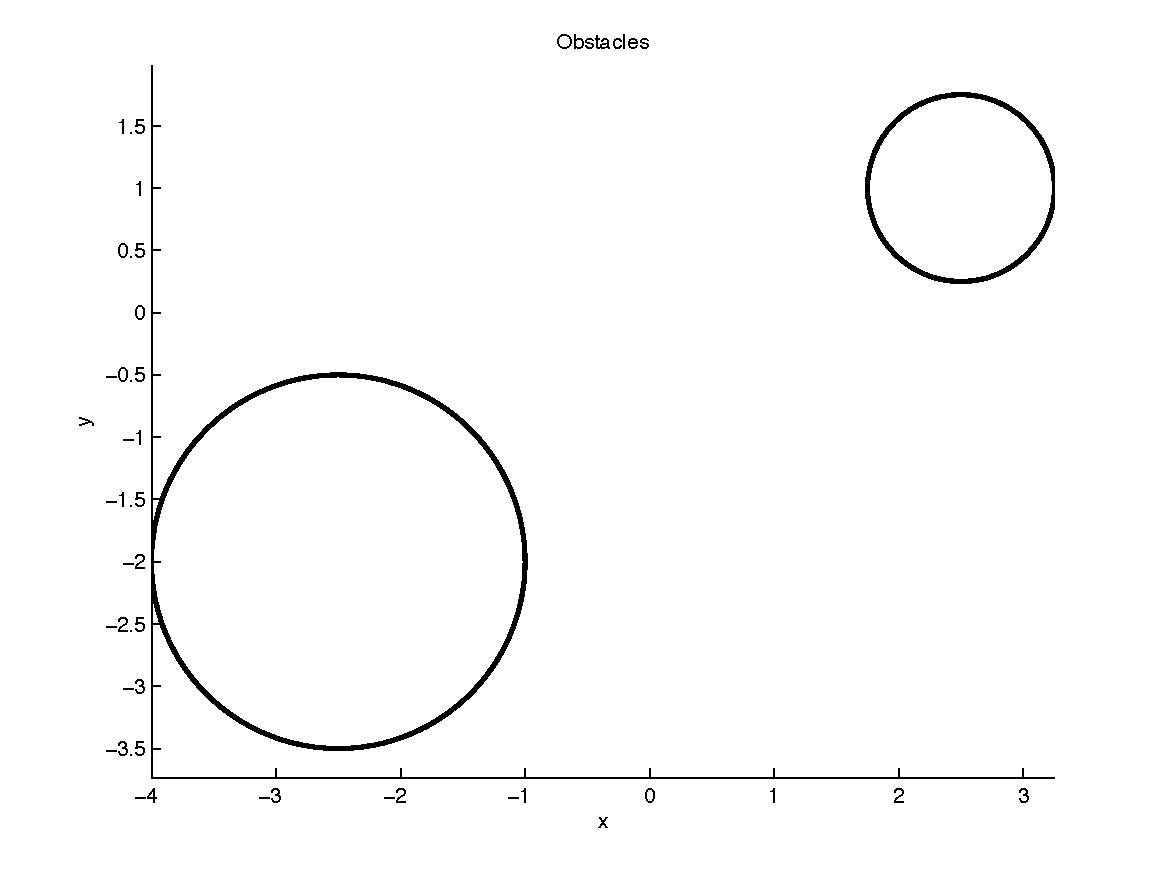
\includegraphics[width=0.45\textwidth]{img/install/obstacles.pdf}}
\subfigure[Absolute value of the total field]{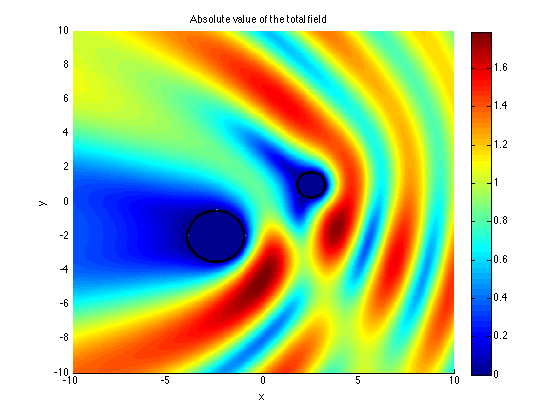
\includegraphics[width=0.45\textwidth]{img/install/absut.png}}
\subfigure[Radar cross section]{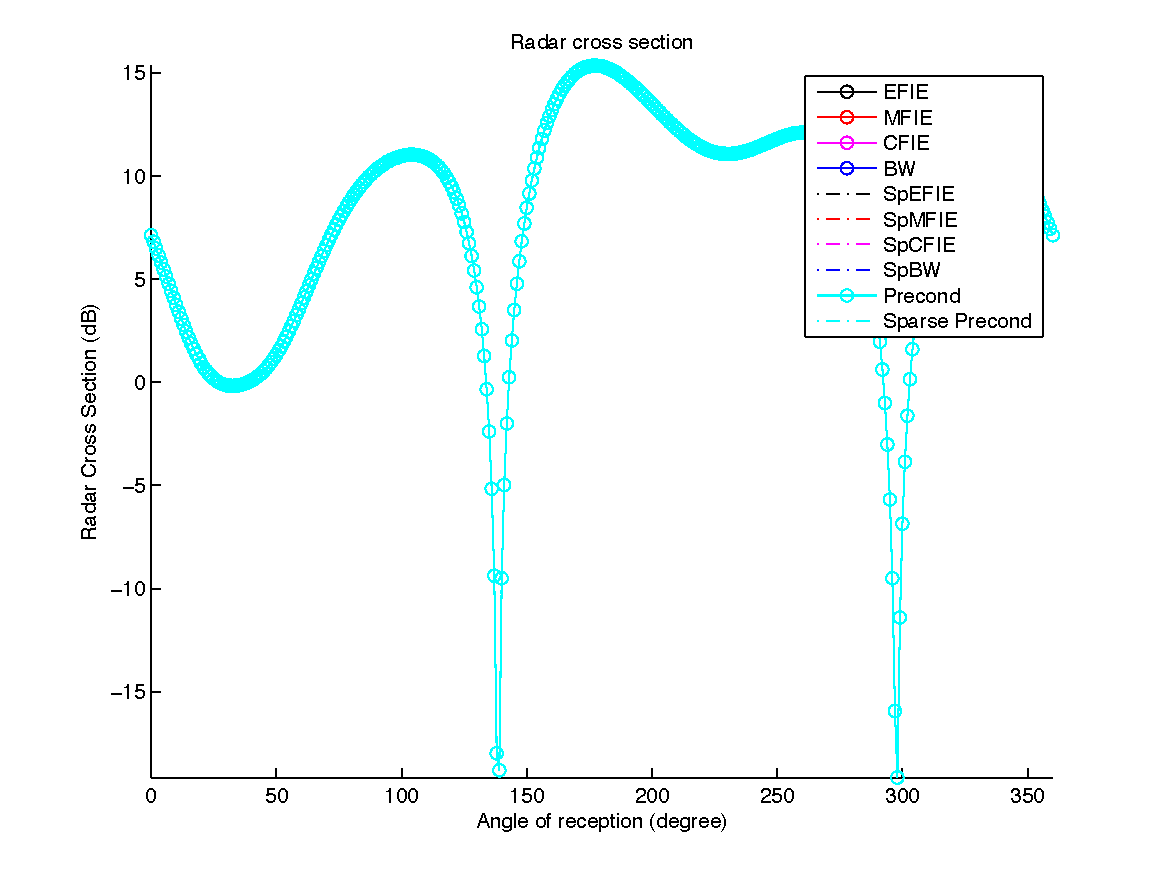
\includegraphics[width=0.45\textwidth]{img/install/rcs.pdf}}
\subfigure[History of convergence of the GMRES]{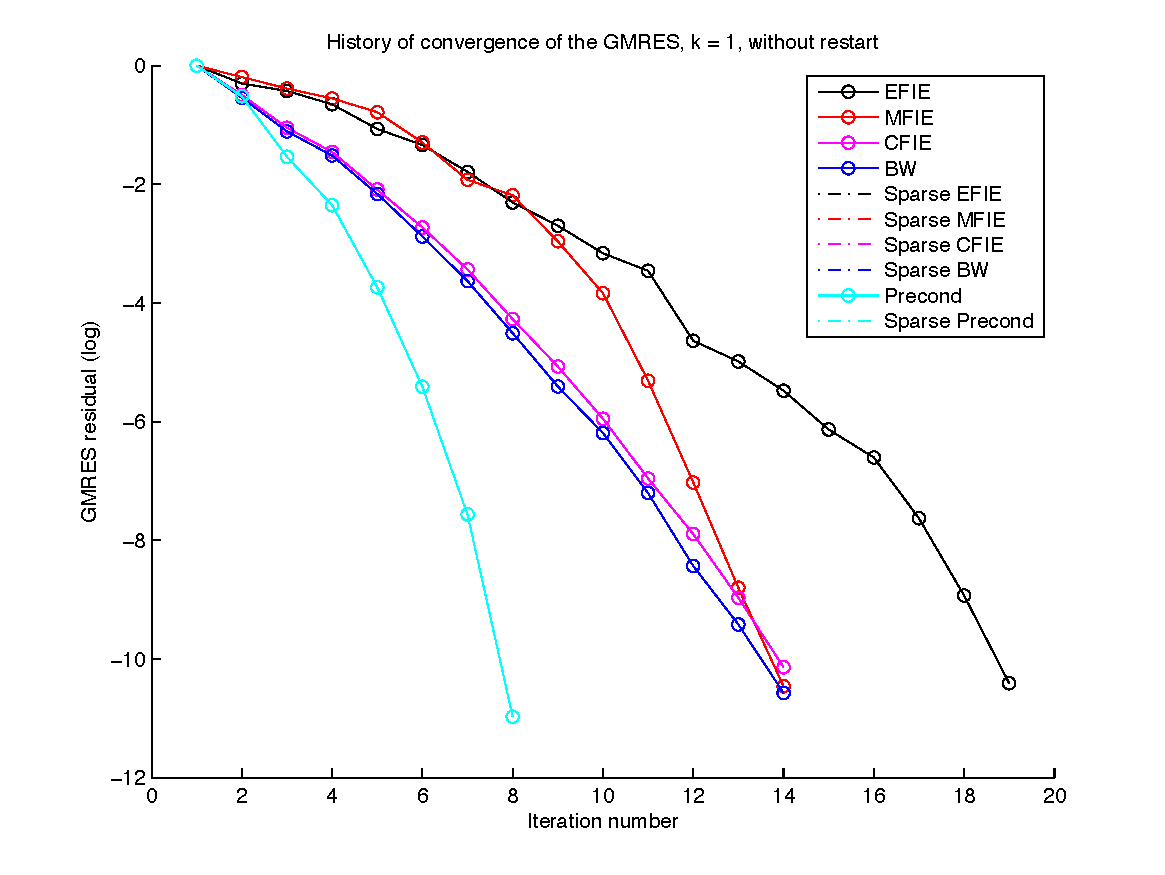
\includegraphics[width=0.45\textwidth]{img/install/gmres.pdf}}
\caption{4 of the different figures that pop up after launching \texttt{BenchmarkDirichlet;}. The first figure shows the two obstacles and the second one the total field. The two others figures, (c) and (d) represent respectively the radar cross section for the different boundary integral equations and the history of convergence of the GMRES solver.}
\end{figure}